\chapter{Ice Reservoirs}

\section{Introduction}

For centuries, in the Himalayan mountain ranges, local cultures have believed that glaciers are alive. And
what’s more, that certain glaciers can have different genders including male and female. These people ‘breed’
new glaciers by grafting together—or marrying—fragments of ice from male and female glaciers, then covering them
with charcoal, wheat husks, cloths, or willow branches so they can reproduce in privacy. These glacierets
transform into fully active glaciers that grow each year with additional snowfall. Those then serve as lasting
reserves of water that farmers can use to irrigate their crops. Over the years, these practices have inspired
other cultures, where people are creating their own artificial ice reservoirs (AIRs) and applying them to solve
serious modern challenges around water supplies.

Take Ladakh, a high-altitude desert region in northern India. It sits in the rain shadow of the Himalayas and
receives on average fewer than ten centimeters of rain/snow per year. As local glaciers shrink because of
climate change, regional water scarcity is increasing. And so, local farmers have started growing their own ice
reservoirs as insurance against this uncertainty. 

Due to low temperatures and high variability of seasonal snow cover
\citep{mukhopadhyayReevaluationSnowmeltGlacial2015}, there is a shortage of water at the onset of the
agricultural season for about two months until a sufficient and reliable supply of meltwater from high altitude
glaciers becomes available. 

AIR serve to bridge this gap in water availability by providing meltwater earlier in the agricultural season.
AIRs do so by exploiting gravity and freezing winter temperatures to amass a seasonal stock of ice. Many types
of AIRs exist. In the past these were built as horizontal ice sheets much higher up the mountains, making them
difficult to manage. Now, as ice cones, they are built next to where the water is needed most, right on the
outskirts of villages, near their fields.

\begin{figure}[t]
\centering
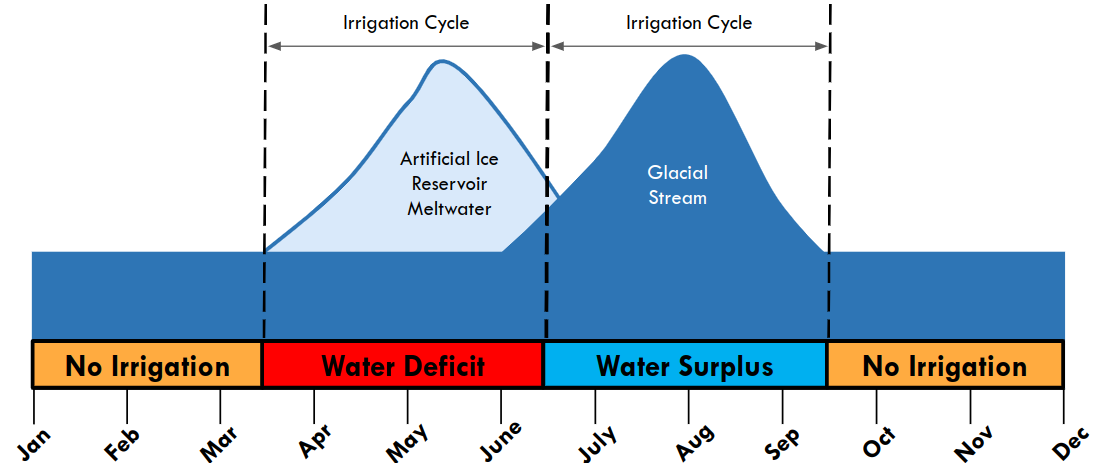
\includegraphics[width=12cm]{Figures/irrigation_cycles.png}

\caption{Seasonal variation in the availability of irrigation water. The graph highlights the crucial role of
AIRs in bridging the phase of water scarcity in spring. Adapted from: \cite{nusserLocalKnowledgeGlobal2016}}

\label{fig:irrigation_cycles}
\end{figure}

While much has been written about the promise of AIRs for irrigation water supply, very little data exists to
support these claims. Published quantifications of their water storage capacity differs between 17,000 and 23500
$m^3$ \citep{norphelSnowWaterHarvesting2015, baglaArtificialGlaciersHelp1998}. Recent research has called for an
examination of their long-term efficacy and their usefulness as climate change adaptation strategies
\citep{clouseLadakhArtificialGlaciers2017}. 

We attempt to address this gap through a measurement campaign of AIRs built in India and Switzerland. This
campaign used drones, flowmeters and weather stations to create a calibration and validation dataset for a mass
and energy balance model. The parameters of the model were calibrated and its ice volume evolution were
validated using this dataset to produced the AIR model. 

The influence of meteorological conditions on AIR water-use efficiency and maximum volume was quantified by
comparing the modelled volume evolution of Indian AIRs and Swiss AIRs.

The influence of the fountain characteristics on AIR water-use efficiency and maximum volume was quantified by
comparing the modelled volume evolution of AIRs produced with different fountain designs and scheduling
strategies.

\section{State of knowledge}

\section{Objectives}

The main objective of this thesis is to quantify the water storage potential of AIRs based on the construction
site and fountain chosen. 


An integrated study approach including field measurements and modelling is applied to
answer the following research questions: 

\begin{itemize}

\item What is the influence of construction location and fountain characteristics on AIR volume evolution? 

\item How can fountain systems be engineered to reduce water loss and maintenance of AIRs?

\end{itemize}

An energy and mass balance model for artificial ice reservoirs was set up to answer the first research question
(paper I and II). Since in-situ measurements were required to run this model, a measurement campaign was
executed in Switzerland and India during the past 4 winters. These datasets provided the necessary input,
calibration and validation data to model the evolution of AIRs and study their sensitivity to meteorological
conditions (paper II). 

A weather-sensitive construction strategy was developed to answer the second research question. This
construction strategy employed fountains whose discharge rate was regulated by automation system using the AIR
model developed before. This weather-sensitive construction strategy was compared with the traditional
construction strategy to quantify its advantages and disavantages (paper III).

\section{Structure}

Chapter 1 introduces the motivation of this work and provides a summary of the state of knowledge about AIRs
prior to this thesis. Chapter 2 describes the origins of this technology as a religious practice. Chapter 3
gives an overview about the study sites and introduces the different field techniques applied. The influence of
the construction location through its meteorological and topographical conditions are presented in Chapter 4.
The enginnering design of AIR technologies are showcased in Chapter 5 along with suggestions for their
improvement. Capter 6 concludes the thesis with a synthesis and future outlook. Papers I, II and III are
included in the Appendix.


